% !TeX program = lualatex
% !TeX root = luaking.tex
% !TeX encoding = UTF-8
% !TeX spellcheck = cs_CZ
%---------------------------------------------------------------------------------------------------
% file fey1ch45.tex
%---------------------------------------------------------------------------------------------------
%=========================== Kapitola: Ilustrace termodynamiky ====================================
\setchaptertoc
\chapter{Ilustrace termodynamiky}\label{fyz:IchapXLV}
  \section{Vnitřní energie}\label{fyz:IchapXLVsecI}
    Termodynamika je poměrně těžká a složitá ve svých aplikacích a bylo by nepřiměřené, kdybychom se
    v tomto kurzu pouštěli při těchto aplikacích příliš do hloubky. je velmi důležitá pro inženýry a
    chemiky, Zájemci se o ní mohou poučit ve fyzikální chemii nebo inženýrské termodynamice.
    Existuje mnoho dobrých příruček, jako např. Zemanskyho „Teplo a termodynamika“, 
    \begin{itemize}[noitemsep]
      \item Úvod do fyziky v řešených příkladech - (\cite{Havrankova1995}).
      \item Fyzika - Vysokoškolská učebnice obecné fyziky - (\cite{Halliday2001}).
      \item Úvod do fyziky v řešených příkladech - (\cite{Havrankova1995}).
      \item Fundamentals of Thermodynamic - (\cite{Borgnakke2012}).
    \end{itemize}
    v nichž se o termodynamice dozvíme hodně. 

    Termodynamika je tak složitá, protože jednu věc můžeme popsat mnoha způsoby. Chceme-li popsat
    chování plynu, můžeme vycházet z toho, že tlak závisí na teplotě a na objemu nebo z toho, že
    objem závisí na teplotě a tlaku. Zajímáme-li se o vnitřní energii \(U\), můžeme vycházet z toho,
    že závisí na teplotě a objemu, ale proměnné si můžeme zvolit i jinak a pak můžeme vycházet z
    toho, že závisí na teplotě a tlaku nebo na tlaku a objemu apod. V poslední kapitole jsme mluvili
    i jiné funkci teploty a objemu, kterou jsme nazývali entropie a můžeme sestrojit ještě mnoho
    jiných funkcí těchto proměnných: například \(U - TS\) je funkcí teploty a objemu. Máme tedy
    mnoho různých veličin, jež mohou být funkcemi rozmanitých kombinací proměnných. Abychom
    nekomplikovali situaci, budeme v této kapitole uvažovat jako nezávisle proměnné teplotu a objem.
    Chemici používají jako nezávislé proměnné teplotu a tlak, protože se snáze měří a ovládají v
    chemických experimentech, ale my budeme v celé kapitole používat teplotu a objem až na jednu
    výjimku, když budeme vysvětlovat, jak se uskutečňuje transformace na chemický systém proměnných.
    
    Budeme tedy uvažovat jen jeden systém nezávislých proměnných: teplotu a objem. Dalším
    omezením bude to, že se budeme zajímat jen o dvě závislé funkce: o vnitřní energii a tlak. O
    ostatních funkcích nebudeme mluvit, neboť je lze odvodit z uvedených dvou funkcí. I přes tato
    omezení je termodynamika stále dost obtížný předmět, i když už ne tolik.

    \begin{figure}[ht!] %\ref{fyz:fig463}
      \centering
      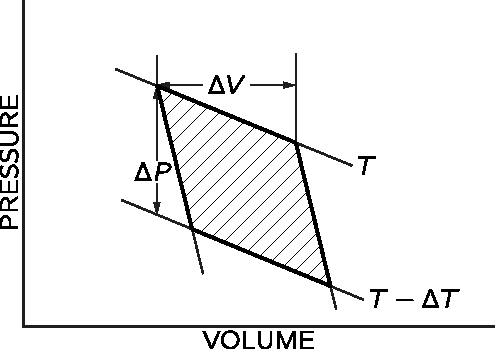
\includegraphics[width=0.7\linewidth]{fyz_fig463.pdf}
      \caption{p-V diagram Carnotova cyklu. Křivky označené \(T\) a \(\Delta T\) jsou izotermy,
               strmější křivky jsou adiabaty. A \(V\) je objemová změna plynu, jemuž bylo při
               konstantní teplotě dodáno teplo \(\Delta\). \(\Delta p\) je změna tlaku plynu, když
               se při konstantním objemu změnila teplota z hodnoty \(T\) na hodnotu \(T - \Delta
               T\). (\cite[s.~615]{Feynman01})}
      \label{fyz:fig463}
    \end{figure}

    \begin{figure}[ht!] %\ref{fyz:fig464}
      \centering
      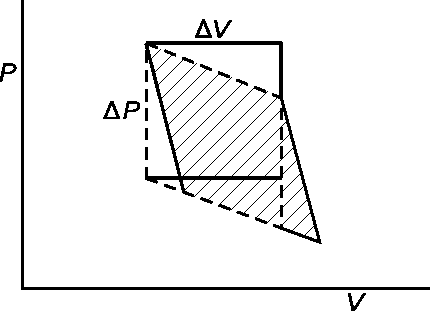
\includegraphics[width=0.7\linewidth]{fyz_fig464.pdf}
      \caption{ 
               (\cite[s.~616]{Feynman01})}
      \label{fyz:fig464}
    \end{figure}

  \section{Aplikace}\label{fyz:IchapXLVsecII}
  \section{Clasiova-Clapeyronova rovnice}\label{fyz:IchapXLVsecIII}
  \section{Příklady a cvičení}\label{fyz:IchapXLVsecIV}



    \begin{figure}[ht!] %\ref{fyz:fig465}
      \centering
      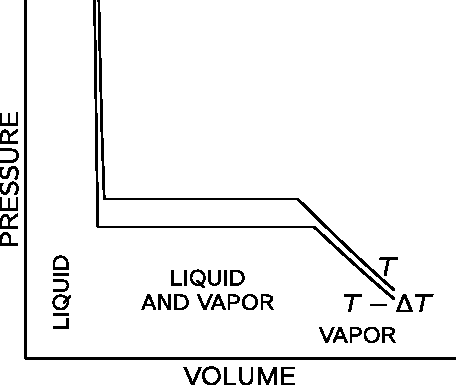
\includegraphics[width=0.7\linewidth]{fyz_fig465.pdf}
      \caption{ 
               (\cite[s.~707]{Feynman01})}
      \label{fyz:fig465}
    \end{figure}

    \begin{figure}[ht!] %\ref{fyz:fig466}
      \centering
      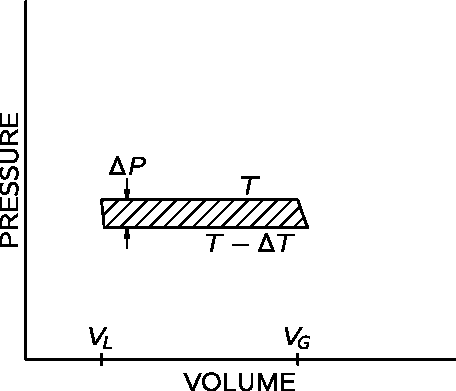
\includegraphics[width=0.7\linewidth]{fyz_fig466.pdf}
      \caption{ 
               (\cite[s.~707]{Feynman01})}
      \label{fyz:fig466}
    \end{figure}
    \todo[inline]{Kapitola fey1ch45 je zcela prázdná, pouze obrázky} 
%---------------------------------------------------------------------------------------------------